%%%%%%%% ICML 2023 EXAMPLE LATEX SUBMISSION FILE %%%%%%%%%%%%%%%%%

\documentclass{article}

% Recommended, but optional, packages for figures and better typesetting:
\usepackage{microtype}
\usepackage{graphicx}
\usepackage{subcaption}
\usepackage{booktabs} % for professional tables

\usepackage{tikz}
% Corporate Design of the University of Tübingen
% Primary Colors
\definecolor{TUred}{RGB}{165,30,55}
\definecolor{TUgold}{RGB}{180,160,105}
\definecolor{TUdark}{RGB}{50,65,75}
\definecolor{TUgray}{RGB}{175,179,183}

% Secondary Colors
\definecolor{TUdarkblue}{RGB}{65,90,140}
\definecolor{TUblue}{RGB}{0,105,170}
\definecolor{TUlightblue}{RGB}{80,170,200}
\definecolor{TUlightgreen}{RGB}{130,185,160}
\definecolor{TUgreen}{RGB}{125,165,75}
\definecolor{TUdarkgreen}{RGB}{50,110,30}
\definecolor{TUocre}{RGB}{200,80,60}
\definecolor{TUviolet}{RGB}{175,110,150}
\definecolor{TUmauve}{RGB}{180,160,150}
\definecolor{TUbeige}{RGB}{215,180,105}
\definecolor{TUorange}{RGB}{210,150,0}
\definecolor{TUbrown}{RGB}{145,105,70}

% hyperref makes hyperlinks in the resulting PDF.
% If your build breaks (sometimes temporarily if a hyperlink spans a page)
% please comment out the following usepackage line and replace
% \usepackage{icml2023} with \usepackage[nohyperref]{icml2023} above.
\usepackage{hyperref}


% Attempt to make hyperref and algorithmic work together better:
\newcommand{\theHalgorithm}{\arabic{algorithm}}

\usepackage[accepted]{icml2023}

% For theorems and such
\usepackage{amsmath}
\usepackage{amssymb}
\usepackage{mathtools}
\usepackage{amsthm}

% if you use cleveref..
\usepackage[capitalize,noabbrev]{cleveref}

%%%%%%%%%%%%%%%%%%%%%%%%%%%%%%%%
% THEOREMS
%%%%%%%%%%%%%%%%%%%%%%%%%%%%%%%%
\theoremstyle{plain}
\newtheorem{theorem}{Theorem}[section]
\newtheorem{proposition}[theorem]{Proposition}
\newtheorem{lemma}[theorem]{Lemma}
\newtheorem{corollary}[theorem]{Corollary}
\theoremstyle{definition}
\newtheorem{definition}[theorem]{Definition}
\newtheorem{assumption}[theorem]{Assumption}
\theoremstyle{remark}
\newtheorem{remark}[theorem]{Remark}

% Todonotes is useful during development; simply uncomment the next line
%    and comment out the line below the next line to turn off comments
%\usepackage[disable,textsize=tiny]{todonotes}
\usepackage[textsize=tiny]{todonotes}


% The \icmltitle you define below is probably too long as a header.
% Therefore, a short form for the running title is supplied here:
\icmltitlerunning{Project Report Template for Data Literacy 2023/24}

\begin{document}

\twocolumn[
\icmltitle{A Data-Driven Perspective on Human Error as a Cause of Fatal Traffic Accidents}


% It is OKAY to include author information, even for blind
% submissions: the style file will automatically remove it for you
% unless you've provided the [accepted] option to the icml2023
% package.

% List of affiliations: The first argument should be a (short)
% identifier you will use later to specify author affiliations
% Academic affiliations should list Department, University, City, Region, Country
% Industry affiliations should list Company, City, Region, Country

% You can specify symbols, otherwise they are numbered in order.
% Ideally, you should not use this facility. Affiliations will be numbered
% in order of appearance and this is the preferred way.
\icmlsetsymbol{equal}{*}

\begin{icmlauthorlist}
\icmlauthor{Leon Trochelmann}{equal,first}
\icmlauthor{Jonathan Ranck}{equal,second}
\icmlauthor{Paul-Henrik Heilmann}{equal,third}
\icmlauthor{Filippo Albani}{equal,fourth}
\end{icmlauthorlist}

% fill in your matrikelnummer, email address, degree, for each group member
\icmlaffiliation{first}{Matrikelnummer 6646000, leon.trochelmann@student.uni-tuebingen.de, MSc Machine Learning}
\icmlaffiliation{second}{Matrikelnummer 6230070, jonathan.ranck@student.uni-tuebingen.de, BSc Physics}
\icmlaffiliation{third}{Matrikelnummer 16648314, paul-henrik.heilmann@student.uni-tuebingen.de, MSc Machine Learning}
\icmlaffiliation{fourth}{Matrikelnummer 6638113, filippo.albani@student.uni-tuebingen.de, MSc Physics}

% You may provide any keywords that you
% find helpful for describing your paper; these are used to populate
% the "keywords" metadata in the PDF but will not be shown in the document
\icmlkeywords{Human Error, Transportation, Analysis, Accidents}

\vskip 0.3in
]

% this must go after the closing bracket ] following \twocolumn[ ...

% This command actually creates the footnote in the first column
% listing the affiliations and the copyright notice.
% The command takes one argument, which is text to display at the start of the footnote.
% The \icmlEqualContribution command is standard text for equal contribution.
% Remove it (just {}) if you do not need this facility.

%\printAffiliationsAndNotice{}  % leave blank if no need to mention equal contribution
\printAffiliationsAndNotice{\icmlEqualContribution} % otherwise use the standard text.


\begin{abstract}
%% Put your abstract here. Abstracts typically start with a sentence motivating why the subject is interesting. Then mention the data, methodology or methods you are working with, and describe results. 
%X is a widely used technique, but can’t do Y. We show that X can actually be interpreted as Z, thus the wonderful technique known as $Z_Y$ can be applied to X to do Y. This means that X can now also be applied/scaled/extended to do various cool things. We demonstrate this in several experiments on real-world data from the domain of D.

Human error in motor vehicle driving, historically distinguished from mechanical errors, faces evolving considerations, particularly in the era of automated vehicles. This study introduces a new data-driven perspective on human error based on the FARS2021National dataset of fatal U.S. traffic accidents. Our analysis reveals a high occurrence of drivers within these accidents being subject to preventable human error, also demonstrating strong correlations with driver demographics and the time of the accident. The high incidence of preventable risk factors in fatal accidents underscores the need for new solutions to enhance road safety in the United States.

\end{abstract}


\section{Introduction}\label{sec:intro}

%% Motivate the problem, situation or topic you decided to work on. Describe why it matters (is it of societal, economic, scientific value?). Outline the rest of the paper (use references, e.g.~to \Cref{sec:methods}: What kind of data you are working with, how you analyse it, and what kind of conclusion you reached. The point of the introduction is to make the reader want to read the rest of the paper.

Human error is a contested term with several accepted definitions \citep{reason2000human, woods2017behind, strauch2017investigating}. In the context of motor vehicle driving it has traditionally been used to differentiate from mechanical error \citep{stanton2009human}, but for example, in the modern context of automated motor vehicles, we may also be interested in considering errors that are specific to human drivers.
\\
In this work, we introduce a new data-driven definition of preventable human error, allowing us to differentiate these human errors from those that may be consequences of the distinct challenges of the driving scenario \citep{guanetti2018control}. We base our definition on the FARS2021National dataset \citep{fars} of fatal traffic accidents in the United States of America and analyse the incidence of preventable human error within it. 
\\
Our results show that an overall high percentage of drivers involved in fatal traffic accidents in the United States were subject to preventable human error. We also observe a strong correlation of such human error with the demographics of the involved drivers and the time of day of the accident.
\\
Ultimately, these results reflect a significant number of potentially avoidable traffic fatalities, presenting evidence of the shortcomings of human drivers that motivate improvements of road traffic safety in the United States.

% Section Introduction:
% - (status quo) Mention that self-driving cars are often motivated by an assumption that car accidents are avoidable and caused by "human error"
% - (problem with the status quo) However, human error is never clearly defined and claims that "90% of car accidents are caused by human error" have no basis to substantiate them
% - (proposed improvment) This is where our project comes in, offering a way to quantify certain preventable human error of which we can be sure that it would not be made by automated cars
% - Outline the paper
%     - Mention which data was used and to what end
%     - Mention which methods were used and to what end
% - Very briefly summarise the takeaways from the results and their implication (contributions)

% From lecture notes:
% - Motivate the idea and the contributions
% - Would be good to have a lot of citations to undermine importance 
%	(note: scholar has a few papers on human error in general, 
%	there's a paper on the difficulties of making a good human error model,
% 	and one about motorcycles)
% - Promise, don't explain

% There is one key paper to reference: "Human error taxonomies applied to driving" on scholar
% - 15 years old, and analysis of error frequency based on data that is almost 50 years old
% - attempts very complex
% - might be able to connect this to the paper on the difficulties of making a useful error model

\section{Data and Methods}\label{sec:methods}
We introduce the dataset we considered for our analysis and show how it leads to our definition of preventable human error. This definition is motivated by several factors which we explain in detail, followed by a description of our analysis.


\subsection{Dataset}
Out of the many possible choices for a dataset on car accidents, we decided to use the FARS2021National dataset by the United States of America's National Highway Traffic Safety Administration. The FARS (Fatality Analysis Reporting System) aims to register all fatal car accidents that occur in the USA in any given year.
\\
FARS captures a large amount of information about each accident, including information about all persons and vehicles involved in the accident, as well as the circumstances of the accident itself. Figure \ref{fig:cases-fars} illustrates how the recorded cases are distributed between the different states in the U.S. in the year 2021.
\begin{figure}[ht]
	\vskip 0.2in
	\begin{center}
		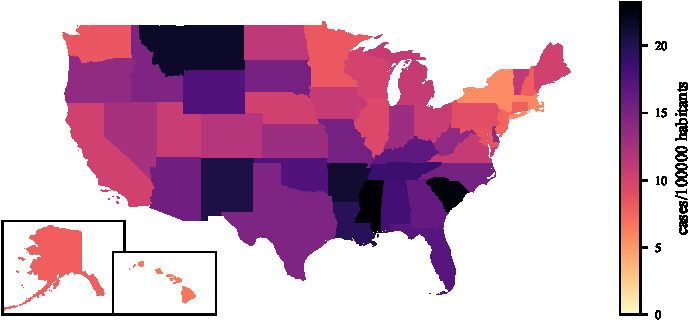
\includegraphics[width = \columnwidth]{plots/cases-fars}
		\caption{Cases of road traffic fatalities in the United States of America in the year 2021 grouped by state and normed by population density.}
		\label{fig:cases-fars}
	\end{center}
	\vskip -0.2in
\end{figure}
The numbers for U.S. population density in that year were obtained from the COVID-19 Open-Data database \cite{google}. With a total of 39508 cases, the FARS dataset presents a rich body of information upon which we base our analysis.
\\
Zoning in on fatal car accidents explicitly is a useful abstraction, as it reduces ambiguity over what constitutes a crash.
\subsection{Defining Preventable Human Error}
To analyse preventable human error, we define it based on a selection of variables that we consider to both reflect error and arise from the human condition specifically. This selection notably excludes risk factors that may not be preventable, such as disabilities. It furthermore disregards risk factors that do not arise from the human condition, such as the weather.\\
Finally, we choose a conservative approach of only selecting risk factors which are generally known to cause many traffic accidents. While these risk factors are not guaranteed to be the true underlying cause of the accident, they can generally be accepted as likely causes.
\\
Specific to FARS2021National we choose the variables speeding, driving without a valid license and driving under the influence to constitute preventable human error. Figure \ref{fig:drivers-err-overlap} illustrates the total number of records that have these attributes and the overlap between the variables.

\begin{figure}[ht]
	\vskip 0.2in
	\begin{center}
		\centerline{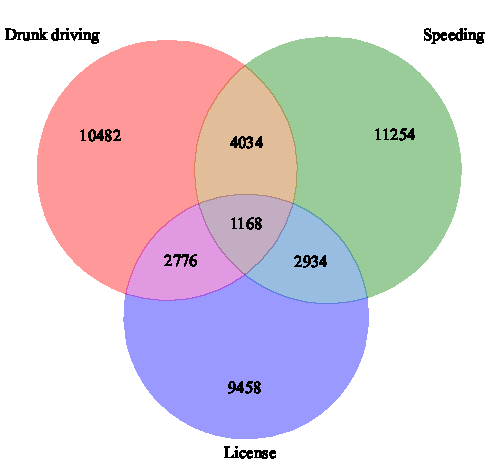
\includegraphics[width=0.49\columnwidth]{plots/drivers-err-overlap}}
		\caption{driver counts for the three variables we consider as preventable human error in FARS2021National.}
		\label{fig:drivers-err-overlap}
	\end{center}
	\vskip -0.2in
\end{figure}

First, we consider a driver record as speeding if the driver went over the speed limit. Second, we consider it to be driving without a license if the driver did not have a valid license. Third, we consider driving under the influence, subject to the judgement of law enforcement. Finally, we introduce preventable human error as a new variable that is TRUE if one of these indicators is given and FALSE otherwise. We will consider only this definition of preventable human error in our analysis.
\\
FARS2021National includes several records where the value of one or more of these variables is missing, of which 3558 were related to speed, 0 to drinking and 2410 to unlicensed driving. For our analysis, we treated all such records as not speeding/drinking/unlicensed driving to preserve the conservative nature of our estimate.
\section{Experiments and Results}\label{sec:results}
To demonstrate the significance of preventable human error and show how it interacts with other variables, we analyse rates of occurrence within the total set of drivers involved in fatal accidents. First, we analyse the total occurrence of preventable human error in our dataset. Second, we investigate how preventable human error is correlated with other variables.
\\
The FARS datasets contain a wide range of variables, many of which have no significant correlation with human error. We present several significant correlations our analysis yielded, but we do not claim completeness. A full correlation analysis with every variable in the FARS is beyond the scope of this work.
\subsection{Occurrence}
Figure \ref{fig:incidence} illustrates the general occurrence of preventable human error.
\begin{figure}[ht]
	\vskip 0.2in
	\centering
		\begin{subfigure}[ht]{0.49\columnwidth}
			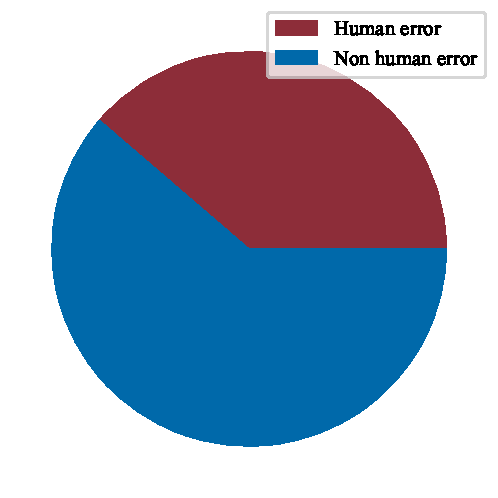
\includegraphics[width=\columnwidth]{plots/err-incidence-total}
			\caption{Incidence of drivers subject to preventable human error.}
			\label{fig:err-incidence-total}
		\end{subfigure}
		\hfill
		\begin{subfigure}[ht]{0.49\columnwidth}
			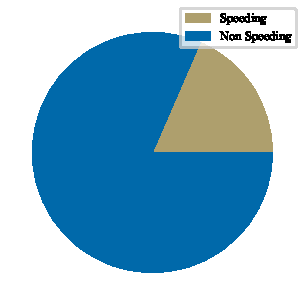
\includegraphics[width=\columnwidth]{plots/err-incidence-speeding}
			\caption{Incidence of drivers subject to speeding.}
			\label{fig:err-incidence-speeding}
		\end{subfigure}

		\vskip\baselineskip
		\begin{subfigure}[ht]{0.49\columnwidth}
			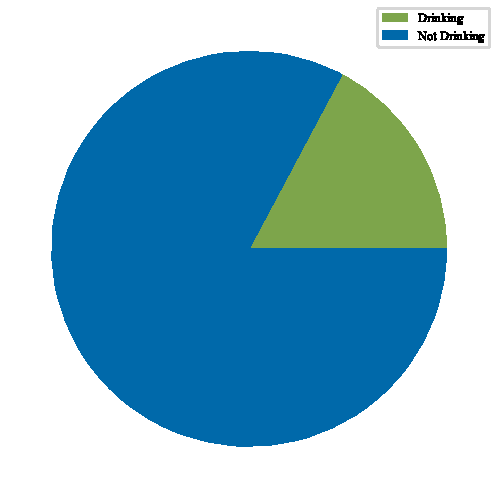
\includegraphics[width=\columnwidth]{plots/err-incidence-drinking}
			\caption{Incidence of drivers subject to drinking.}
			\label{fig:err-incidence-drinking}
		\end{subfigure}
		\hfill
		\begin{subfigure}[ht]{0.49\columnwidth}
			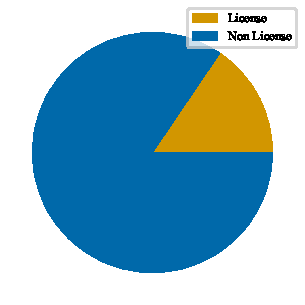
\includegraphics[width=\columnwidth]{plots/err-incidence-license}
			\caption{Incidence of drivers subject to unlicensed driving.}
			\label{fig:err-incidence-license}
		\end{subfigure}
	\caption{Incidence of preventable human errors as a percentage out of the total set of drivers.}
	\label{fig:incidence}
	\vskip 0.2in
\end{figure}
\\
Figure \ref{fig:err-incidence-total} demonstrates approximately 38.70\% of all drivers in our dataset to be subject to preventable human error. For the individual variables, we observe ca. 18.48\% of cases to be subject to speeding, 17.21 \% to drinking and 15.53\% to unlicensed driving as seen in figures \ref{fig:err-incidence-speeding}, \ref{fig:err-incidence-drinking} and \ref{fig:err-incidence-license} respectively.

\subsection{Correlations}
We find that preventable human error is strongly correlated with the demography of the drivers and the time of the accident.
\\
We begin by demonstrating the demographics of preventable human error by conditioning on age and sex. We plot the percentages of driver records subject to human errors as an overlapping violin plot with binned age groups for the sake of readability, displayed in figure \ref{fig:err-demography}. We also show the amounts of records attributed to each age group for context.
\begin{figure}[ht]
	\vskip 0.2in
	\begin{center}
		\centerline{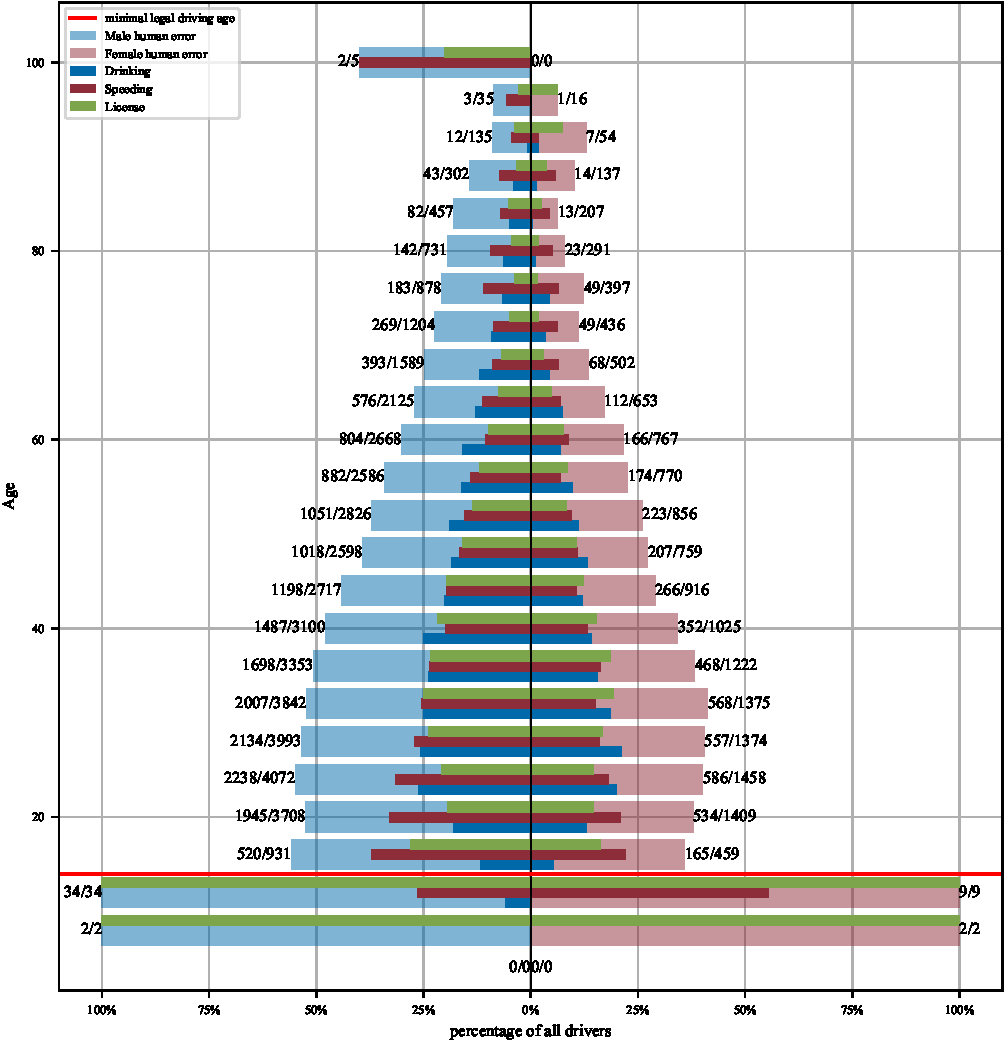
\includegraphics[width=\columnwidth]{plots/err-demography}}
		\caption{Correlation of preventable human error with age and sex as a percentage of the total set of drivers. The male population is displayed on the left and the female population is on the right. Each type of error is displayed in a different colour. The bin size is 4. The numbers of records considered for each age group are explicitly displayed at the end of the bars, as a fraction of records with preventable human error out of all driver records. The absolute minimum legal driving age of 14 is highlighted in red and located precisely between the respective bins.}
		\label{fig:err-demography}
	\end{center}
	\vskip -0.2in
\end{figure}

Trivially, the rate of preventable human error is 1 for all age groups below the absolute minimum legal driving age in the USA. We observe that the incidence of preventable human error is overall higher in the male population. Additionally, the incidence of preventable human error decreases with older age groups.
\\
We observe different peaks in the percentage and total number of drivers subject to preventable human errors in the male and female populations respectively. The percentage of preventable human error reaches its peak in the 14 to 17 age group for the male population and in the 30 to 33 age group for the female population. Meanwhile, the total number of driver records indicating preventable human error has a peak in the 22 to 25 age group for males and a significantly lower peak again in the 30 to 33 age group for females.\\
There are significantly fewer total drivers subject to preventable human error in the female population as compared to the male population in nearly every age group. Due to the low number of total cases in the 98 to 101 age group, it may be considered an outlier.\\
Regarding the individual error variables, we observe a gradual decrease in the percentage of speeding in older age groups, whereas the percentage of drinking displays a rise and fall. The percentage of unlicensed driving behaves somewhat irregularly, as it displays a series of increases and decreases throughout the age ranges, but ultimately also exhibits the mass of its distribution lying within the younger age groups.\\
\\
The time of day also has a significant correlation with preventable human error. We plot the percentage of drivers subject to preventable human error conditioned on the time of the accident in hourly intervals, displayed in \ref{fig:err-time}. We see a significant increase in drunk driving during the late evening and early night, see figure \ref{fig:err-time-drinking}, whereas speeding and and unlicensed driving are more evenly distributed.
\begin{figure}[ht]
	\vskip 0.2in
	\centering
		\begin{subfigure}[ht]{0.49\columnwidth}
			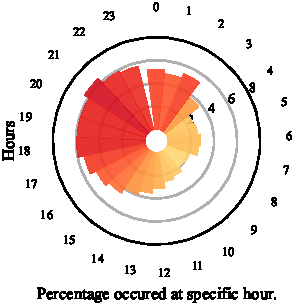
\includegraphics[width=\columnwidth]{plots/err-time-total}
			\caption{Incidence of preventable human error by the time of day.}
			\label{fig:err-time-overall}
		\end{subfigure}
		\hfill
		\begin{subfigure}[ht]{0.49\columnwidth}
			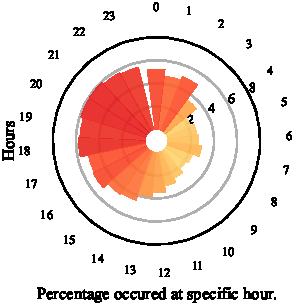
\includegraphics[width=\columnwidth]{plots/err-time-speeding}
			\caption{Incidence of speeding by the time of day.}
			\label{fig:err-time-speeding}
		\end{subfigure}

		\vskip\baselineskip
		\begin{subfigure}[ht]{0.49\columnwidth}
			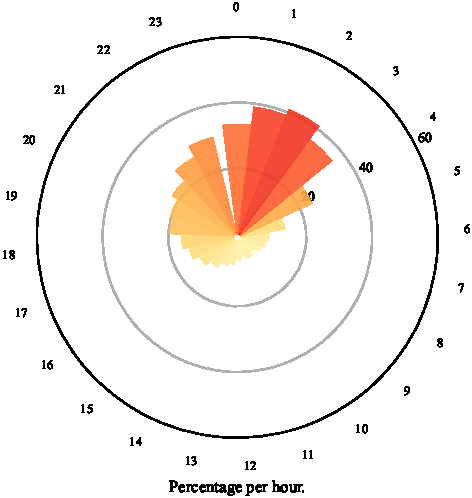
\includegraphics[width=\columnwidth]{plots/err-time-drinking}
			\caption{Incidence of drunk driving by the time of day.}
			\label{fig:err-time-drinking}
		\end{subfigure}
		\hfill
		\begin{subfigure}[ht]{0.49\columnwidth}
			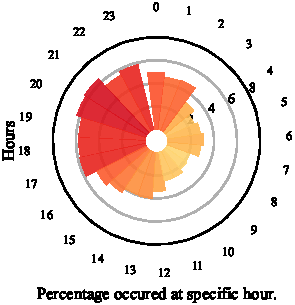
\includegraphics[width=\columnwidth]{plots/err-time-license}
			\caption{Incidence of unlicensed driving by the time of day.}
			\label{fig:err-time-license}
		\end{subfigure}
	\caption{The correlation of time of day in hours with preventable human error as a percentage of the set of all drivers at an hour of the day. The scale is presented through three equidistant circles, each representing a 20\% distance.}
	\label{fig:err-time}
	\vskip 0.2in
\end{figure}
\hfill \break
To examine the overall time distribution of drivers that were subject to preventable human error, we plot the number of drivers and also expand our time intervals to consider the days of the week, seen in figure \ref{fig:time-week}.
\begin{figure}[ht]
	\vskip 0.2in
	\centering
		\begin{subfigure}[ht]{\columnwidth}
			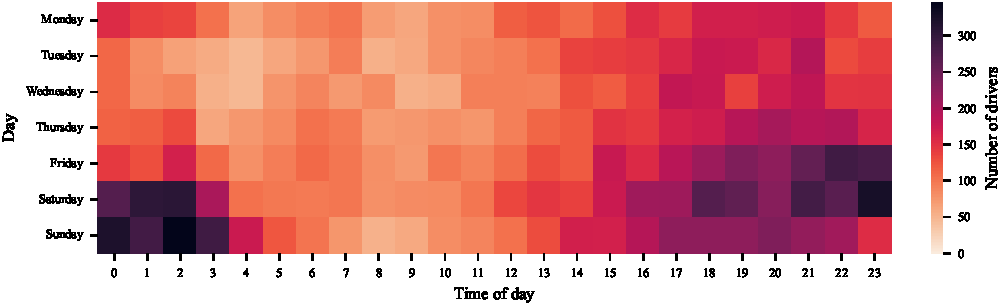
\includegraphics[width=\columnwidth]{plots/err-time-week}
			\caption{Number of drivers involved in fatal accidents and subject to preventable human error.}
			\label{fig:err-time-week}
		\end{subfigure}
		\vskip\baselineskip
		\begin{subfigure}[ht]{\columnwidth}
			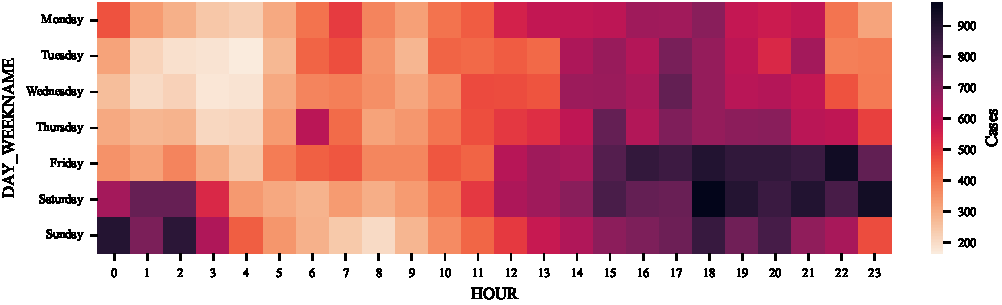
\includegraphics[width=\columnwidth]{plots/drivers-time-week}
			\caption{Numbers of total drivers involved in fatal accidents.}
			\label{fig:drivers-time-week}
		\end{subfigure}
	\caption{The total amounts of drivers involved in fatal accidents plotted by the time of day and day of the week concerning the crash. To visually compensate for the overall difference in the number of drivers, we use the same colour bar over a different range of drivers for the two plots respectively}
	\label{fig:time-week}
	\vskip 0.2in
\end{figure}
\hfill \break
The distribution of drivers subject to preventable human error illustrated in \ref{fig:err-time-week} exhibits a clear similarity to the number of total drivers displayed in figure \ref{fig:drivers-time-week} for reference. Specifically, the distribution exhibits a concentration in the later hours of the day and over the weekend.\\
Comparing the distributions side by side, one can observe that preventable human error is overall less present in the evenings on weekdays but equally concentrated towards the weekend. The distribution of preventable human error also displays less density during the mornings than the overall distribution.
\section{Discussion \& Conclusion}\label{sec:conclusion}
%% Use this section to briefly summarize the entire text. Highlight limitations and problems, but also make clear statements where they are possible and supported by the analysis. 

In this work, we have introduced a data-driven definition of preventable human error and demonstrated its high occurrence based on a vast dataset of fatal car accidents.
\\
Our results show that preventable risk factors have a significant incidence in fatal motor vehicle accidents. They also show that the incidence is strongly correlated with the demography of drivers and the time of the accident.
\\
Due to our conservative approach to variable selection, these rates of occurrence can also be seen as lower bounds on the true rate of irresponsible driving in fatal car accidents, as we did not consider difficult-to-assess factors like road rage and reckless driving.
\\
Our analysis is based on traffic data that stems exclusively from the USA in the year 2021. We conducted our analysis at the federal level, such that the statistics over individual states may differ. Furthermore, different rates of occurrence may come about in other countries or at different points in time.
\\
Overall, the presence of significant quantities of preventable human error motivates changes in the motorway traffic system in the USA, whether these solutions be automotive, legislative or societal. 


\section*{Contribution Statement}

%% Explain here, in one sentence per person, what each group member contributed. For example, you could write: Max Mustermann collected and prepared data. Gabi Musterfrau and John Doe performed the data analysis. Jane Doe produced visualizations. All authors will jointly wrote the text of the report. Note that you, as a group, a collectively responsible for the report. Your contributions should be roughly equal in amount and difficulty.
Leon conceptualised the project, authored the report and assisted with visualisations. Jonathan \ldots Paul \ldots Filippo \ldots
\\


% \section*{Notes} 

% Your entire report has a \textbf{hard page limit of 4 pages} excluding references. (I.e. any pages beyond page 4 must only contain references). Appendices are \emph{not} possible. But you can put additional material, like interactive visualizations or videos, on a githunb repo (use \href{https://github.com/pnkraemer/tueplots}{links} in your pdf to refer to them). Each report has to contain \textbf{at least three plots or visualizations}, and \textbf{cite at least two references}. More details about how to prepare the report, inclucing how to produce plots, cite correctly, and how to ideally structure your github repo, will be discussed in the lecture, where a rubric for the evaluation will also be provided.

\bibliography{bibliography}
\bibliographystyle{icml2023}

\end{document}


% This document was modified from the file originally made available by
% Pat Langley and Andrea Danyluk for ICML-2K. This version was created
% by Iain Murray in 2018, and modified by Alexandre Bouchard in
% 2019 and 2021 and by Csaba Szepesvari, Gang Niu and Sivan Sabato in 2022.
% Modified again in 2023 by Sivan Sabato and Jonathan Scarlett.
% Previous contributors include Dan Roy, Lise Getoor and Tobias
% Scheffer, which was slightly modified from the 2010 version by
% Thorsten Joachims & Johannes Fuernkranz, slightly modified from the
% 2009 version by Kiri Wagstaff and Sam Roweis's 2008 version, which is
% slightly modified from Prasad Tadepalli's 2007 version which is a
% lightly changed version of the previous year's version by Andrew
% Moore, which was in turn edited from those of Kristian Kersting and
% Codrina Lauth. Alex Smola contributed to the algorithmic style files.
